\chapter{\stateoftheartname}

\section{Transformación digital y amenazas emergentes}
La sociedad contemporánea se encuentra inmersa en una profunda
transformación digital impulsada por el avance acelerado de las Tecnologías de la Información y la Comunicación (TIC). Esta evolución ha permitido la interconexión masiva de dispositivos, servicios y sistemas críticos,promoviendo una digitalización sin precedentes en sectores como la banca, la sanidad, el transporte, la defensa o la administración pública. Sin embargo, esta dependencia creciente de las infraestructuras digitales conlleva también un incremento proporcional en la superficie de exposición a amenazas cibernéticas cada vez más sofisticadas y persistentes~\cite{Saeed2023}. 

En este contexto, la ciberseguridad ha pasado de ser un complemento técnico a convertirse en un elemento estratégico para garantizar la continuidad operativa, la privacidad de los usuarios y la integridad de los sistemas. La aparición de tecnologías disruptivas como la computación cuántica está reconfigurando el panorama de la seguridad digital al cuestionar la solidez de los actuales sistemas criptográficos sobre los que se sostiene la protección de la información en la era digital~\cite{Mosca2018}.

La computación cuántica representa un salto cualitativo en el procesamiento
de la información al usar principios de la mecánica cuántica como la
superposición de estados, el entrelazamiento, entre otros. Estas propiedades
permiten resolver problemas imposibles para los ordenadores clásicos, en
tiempos polinómicos. Algoritmos cuánticos como Shor o Grover, ya han demostrado
ser capaces de debilitar los fundamentos de la criptografía de claves públicas
y claves simétricas~\cite{Shor1997}.

Ante este panorama, la necesidad de establecer sistemas de seguridad y comunicación resilientes frente a adversarios cuánticos se vuelve prioritaria. No se trata únicamente de responder a una amenaza futura, sino de anticiparse a escenarios de vulnerabilidad como el denominado “Harvest now, decrypt later”~\cite{Adeola2025}, donde los atacantes interceptan datos cifrados con el objetivo de descifrarlos en el futuro cuando dispongan de ordenadores cuánticos adecuados.

En respuesta, la comunidad científica y los organismos internacionales han impulsado dos grandes líneas complementarias de investigación: por un lado, las comunicaciones cuánticas seguras, basadas en principios físicos que garantizan la detección de cualquier intento de interceptación (como ocurre en la Distribución Cuántica de Claves); y por otro, la criptografía post-cuántica, que busca diseñar algoritmos resistentes a ataques cuánticos que puedan ser ejecutados en sistemas clásicos~\cite{Aquina2025}.

Este trabajo se enmarca en el objetivo de revisar sistemáticamente los
avances, desafíos y sinergias entre ambas disciplinas, proporcionando una
visión global que permita identificar las mejores estrategias de transición
hacia una ciberseguridad e infraestructura de comunicaciones adaptadas a la era
cuántica.


\section{Evolución histórica}

\subsection{Orígenes y evolución de las comunicaciones cuánticas}
Las comunicaciones cuánticas surgen como combinación entre la física
cuántica y las tecnologías de la información, con el objetivo principal de
garantizar la transmisión segura de información usando las propiedades de los
sistemas cuánticos. Para comprender su origen es necesario remontarse a los
fundamentos de la mecánica cuántica, una teoría física instaurada a comienzos
del siglo XX para describir el comportamiento de la materia y energía en
escalas subatómicas.

Sin embargo, no fue hasta finales del siglo XX cuando se planteó por
primera vez el concepto de utilizar propiedades cuánticas para la trasmisión de
información, surgiendo la disciplina que hoy en día se conoce como comunicaciones
cuánticas.

El año 1984 es ampliamente reconocido por la literatura especializada, dado
que se publicaron los primeros trabajos pioneros que sentaron las bases de la criptografía y la comunicación cuántica, marcando un hito histórico para esta disciplina. Charles H. Bennett y Gilles Brassard publicaron el protocolo BB84~\cite{EITCA_BB84}, considerado el primer esquema funcional de Distribución Cuántica de Claves (QKD). Este protocolo permite a dos partes establecer una clave secreta
compartida con la garantía de que cualquier intento de interceptación por parte
de un tercero será detectado debido a la perturbación inducida en los qubits
durante la transmisión.

Posteriormente, en 1991 Artur Ekert propuso el protocolo E91 basado en la
seguridad de la distribución de claves en las correlaciones cuánticas del
principio físico de entrelazamiento~\cite{Ekert1991}. Lo innovador de su propuesta era la herramienta matemática empleada, conocida como las desigualdades de Bell, para verificar la ausencia de intrusos en el canal de comunicación, idea fundamentada en estudios previos realizados por Alain Aspect durante los años 80~\cite{Aspect1982}.

A partir de los años 2000, la experimentación con la Distribución Cuántica
de Claves (QKD) avanzó significativamente, logrando transmisiones a distancias
crecientes mediante fibras ópticas, canales de espacio libre e incluso enlaces
satelitales. Un hito reciente y de gran relevancia fue el lanzamiento del
satélite Micius por parte de China en 2016, logrando transmisiones QKD a escala
continental, estableciendo un paso más hacia una futura red de Internet
cuántico global~\cite{Yin2017}.

\subsection{Orígenes y evolución de la ciberseguridad en la era post-cuántica}
El concepto de ciberseguridad post-cuántica surge como respuesta directa al
desarrollo de la computación cuántica y la amenaza que supone por su facilidad
para comprometer los fundamentos de los sistemas criptográficos tradicionales.
Desde mediados del siglo XX, gran parte de la infraestructura digital global ha
confiado su seguridad a algoritmos de criptografía de claves públicas como RSA,
ECC y DSA, cuya robustez se sustenta en la dificultad computacional de problemas
matemáticos complejos.

Sin embargo, en 1994, el matemático Peter Shor desarrolló un algoritmo cuántico
que puso en duda la seguridad que ofrecían los sistemas criptográficos de la
época, el algoritmo de Shor~\cite{Shor1997}. Este algoritmo demostró que un ordenador cuántico
suficientemente potente podría resolver estos problemas matemáticos en tiempo
polinómico, poniendo en riesgo la confidencialidad y autenticidad de la
información cifrada bajo los algoritmos tradicionales.

Aunque aún no existen ordenadores cuánticos capaces de ejecutar plenamente
este algoritmo, la amenaza sí es real. Durante los años 2000, comenzaron a
crearse nuevas líneas de investigación
centradas en diseñar algoritmos criptográficos capaces de resistir ataques realizados
con tecnología cuántica. A este nuevo campo se le denominó como Post-Quantum Cryptography
(PQC)~\cite{NIST_WhatIsPQC}.

Desde entonces, el foco de la ciberseguridad post-cuántica ha evolucionado de
un problema teórico a una necesidad práctica en la planificación de sistemas a
largo plazo, percibiéndose como una cuestión estratégica a nivel internacional,
incluyendo directrices de migración temprana, evaluaciones de impacto y simulaciones
de escenarios híbridos para prepararse ante un posible salto tecnológico
inminente.

\section{Conceptos físicos fundamentales}

Para comprender el estado del arte actual en ámbitos paralelos como son las
comunicaciones cuánticas y ciberseguridad en la era post-cuántica, es
imprescindible entender primero una serie de conceptos fundamentales asociados
a la física cuántica y criptografía moderna que sustentan las bases del
desarrollo teórico de ambas disciplinas.

\subsubsection{Qubits vs. Bits}
A diferencia de la computación clásica, donde la información es
representada en forma de bits, unidades binarias que adoptan uno de los dos
estados posibles: 0 o 1, la computación cuántica utiliza qubits, unidades de
información cuántica que pueden existir en una superposición de estados
simultáneamente. Esto permite que un qubit exista en múltiples estados al mismo
tiempo, formando una combinación lineal de 0 y 1, aumentando así la capacidad
de procesamiento de datos de manera exponencial.

Formalmente, un qubit se describe como:
$$ |\psi\rangle = \alpha|0\rangle + \beta|1\rangle $$
Donde $\alpha$ y $\beta$ son números complejos que representan la amplitud de probabilidad de cada
estado, y cumplen que $|\alpha|^2 + |\beta|^2 = 1$.

Para visualizar esta propiedad de superposición, se utiliza un modelo
geométrico conocido como la esfera de Bloch. En este modelo, cualquier
estado puro de un qubit puede representarse como un punto en la superficie de
una esfera tridimensional. Los estados $|0\rangle$ y $|1\rangle$ se ubican en los
polos norte y sur de la esfera, respectivamente, mientras que los estados en
superposición ocupan posiciones intermedias, determinadas por dos ángulos: $\theta$ (latitud) y $\phi$ (longitud).

% FIGURE I: REPRESENTACIÓN DE BIT VS QUBIT
\begin{figure}[H]
\centering
\caption[Representación de Bit vs Qubit]{
    \vspace{4pt}
    \fontsize{12}{11}\selectfont \\
    Representación de Bit vs Qubit \\[2pt]
    \footnotesize Fuente: Elaboración propia
}
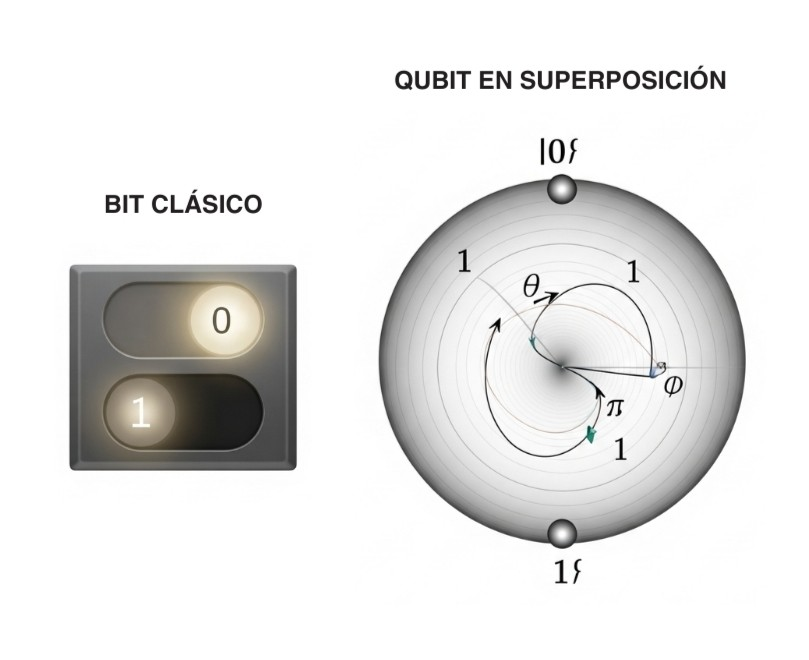
\includegraphics[width=0.58\textwidth]{pictures/Bit_vs_Qbit.jpg}
\label{fig:bit_vs_qubit}
\end{figure}


Además, existen otras propiedades fisicas fundamentales para las comunicaciones cuánticas seguras, como son:

\begin{itemize}
    \item \textbf{Entrelazamiento cuántico:} El entrelazamiento cuántico permite que los qubits estén intrínsecamente correlacionados, de forma que el estado de uno depende instantáneamente del estado del otro, sin importar la distancia que los separe~\cite{Horodecki2009}.
    \item \textbf{No clonación:} El teorema de no clonación establece que no es posible copiar un estado cuántico sin ser perturbado, eliminando por completo la duplicación no autorizada de información, siendo un principio importantísimo en la seguridad de las comunicaciones cuánticas~\cite{Wootters1982}.
\end{itemize}

\section {Comunicaciones Cuánticas y Ciberseguridad Post-Cuántica}
El presente estado del arte aborda de forma conjunta las comunicaciones cuánticas y la ciberseguridad en la era post-cuántica, ya que son dos áreas tecnológicas profundamente interconectadas que evolucionan en paralelo y responden a desafíos comunes. 

Por un lado la ciberseguridad post-cuántica, se centra en diseñar algoritmos criptográficos capaces de resistir la computación cuántica además de protocolos, infraestructuras y marcos normativos que garanticen la integridad, confidencialidad y autenticación de los datos en un escenario donde los algoritmos tradicionales ya no son seguros. Por otro lado, la comunicación cuántica busca transformar la forma en que se transmite la información creando canales de comunicación con un nivel de seguridad inalcanzable por las teorías convencionales. 

Mientras la ciberseguridad post-cuántica protege los datos a nivel lógico, la comunicación lo hace a nivel físico del canal de transmisión. Analizar ambas dimensiones de forma conjunta nos permite comprender mejor panorama post-cuántico emergente, donde la protección de la información, la transmisión segura de datos y la soberanía digital comparten fundamentos, retos y oportunidades comunes.

\subsection{Pilares Tecnológicos y Desarrollo de Infraestructuras Cuánticas}

A continuación se describen algunas de las tecnologías más relevantes que están marcando el desarrollo actual de las disciplinas estudiadas.

\subsubsection{Teletransporte Cuántico} % This will be 4.4.1.1

El teletransporte cuántico es una tecnología que permite transmitir el
estado cuántico completo de una partícula a otra situada a gran distancia. Esta
transferencia no implica el traslado físico de la partícula, sino de su estado
cuántico, es decir, la información cuántica que la describe~\cite{Bennett1993}.

En el proceso de teletransporte cuántico, dos partes (comúnmente llamadas
Alice y Bob) deben compartir previamente un par de partículas entrelazadas. Este entrelazamiento cuántico implica una
correlación entre los estados de ambas partículas, de tal manera que cualquier
medición realizada en una de las partículas afecta instantáneamente al estado
de la otra, sin importar la distancia que las separe.

El proceso se desarrolla en tres pasos clave:
\begin{enumerate}
    \item \textbf{Preparación del entrelazamiento:} Se distribuye un par de partículas entrelazadas entre Alice y Bob.
    \item \textbf{Medición conjunta y comunicación clásica:} Alice recibe una tercera partícula (C), cuyo estado
    cuántico es completamente desconocido y será teletransportado. Para ello,
    realiza una medición conjunta de tipo Bell sobre las partículas (su parte del
    par entrelazado) y C (el estado a transferir). Esta medición destruye el
    estado original de C, en conformidad con el teorema de no clonación cuántica,
    y los resultados generados son enviados a Bob mediante un canal de comunicación
    clásico.
    \item \textbf{Reconstrucción del estado cuántico:} Bob recibe los resultados y aplica una serie de transformaciones cuánticas
    específicas sobre su partícula B, transformándola en una copia idéntica del
    estado original de C. Así se completa el proceso de teletransporte: el estado
    cuántico se ha movido sin que la partícula portadora original lo acompañe
    físicamente.
\end{enumerate}

\begin{figure}[H]
\centering
\caption[Representación Teletransporte cuántico]{
    \vspace{4pt}
    \fontsize{12}{11}\selectfont \\
    Representación Teletransporte cuántico \\[2pt]
    \footnotesize Fuente: Elaboración propia
}
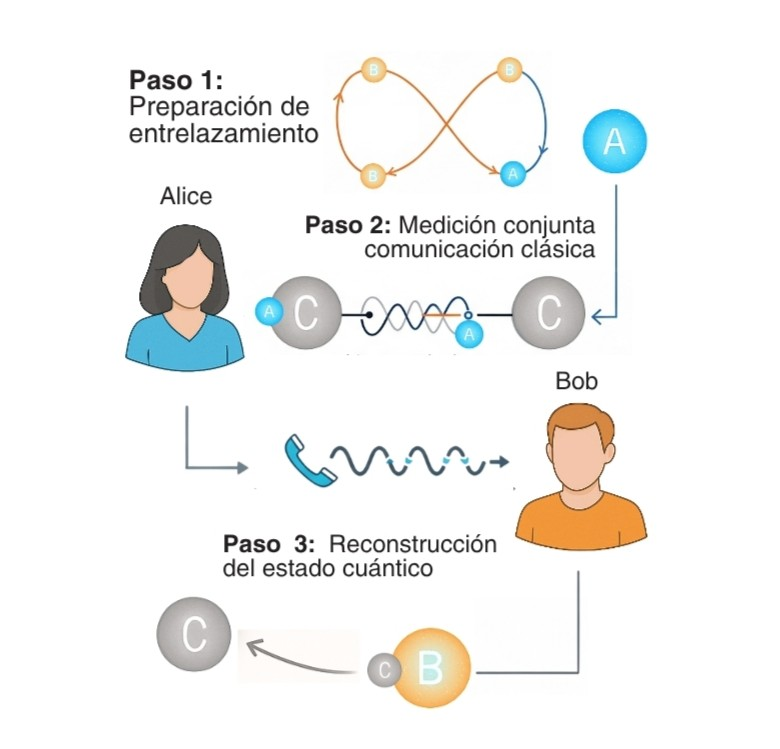
\includegraphics[width=0.58\textwidth]{pictures/Teletransporte_cuantico.jpg}
\label{fig:RepresentacionTeletransporte}
\end{figure}

Este protocolo no permite una comunicación más rápida que la luz, ya que la información final requiere una señal clásica. No obstante, constituye un componente esencial para el futuro de las redes cuánticas distribuidas, los repetidores cuánticos y la computación cuántica escalable, ya que posibilita transmitir estados cuánticos con el máximo grado de fidelidad a distancias arbitrarias.

\subsubsection{Criptografía Cuántica}

La criptografía cuántica se basa en la utilización de estados cuánticos como portadores de la información y transmitir así las claves entre usuarios legítimos a través de canales de comunicación cuánticos.

A diferencia de la criptografía clásica, cuya seguridad depende exclusivamente de la dificultad computacional de resolver ciertos problemas matemáticos, la criptografía cuántica se sustenta bajo los principios de la mecánica cuántica, ofreciendo una seguridad teóricamente inviolable, ya que cualquier intento de interceptación o medición por parte de un tercero altera el estado cuántico del sistema, haciendo posible su detección inmediata.

Cuando un atacante intenta acceder a la información transmitida, necesariamente debe realizar una medición cuántica, lo que interrumpe los estados de superposición o entrelazamiento utilizados en la comunicación. Este tipo de intervención introduce anomalías observables en el canal, como cambios en las tasas de error o correlaciones rotas, lo que permite a los usuarios legítimos detectar la presencia de una intrusión. Así, la criptografía cuántica no impide los intentos de espionaje, pero sí garantiza que cualquier intento sea detectable.
La aplicación más consolidada de la criptografía cuántica es la Distribución Cuántica de Claves (QKD)~\cite{Lo2014}. Este mecanismo no transmite directamente información útil o mensajes cifrados, sino que genera claves simétricas de forma segura, que luego pueden utilizarse en algoritmos de cifrado tradicionales. Su principal fortaleza radica en que la seguridad no depende de supuestos computacionales, sino en la imposibilidad física de medir un estado cuántico sin alterarlo, lo cual deriva del principio de incertidumbre de Heisenberg y del teorema de no clonación.

QKD puede ser implementado a través de fibra óptica, enlaces de espacio libre (FSO) o comunicaciones satelitales, permitiendo alcanzar comunicaciones metropolitanas e incluso a escala global.

Esta tecnología ha sido validada en entornos controlados y desplegada en redes experimentales, como la red cuántica Beijing-Shanghai, una de las primeras redes comerciales de QKD, o las pruebas realizadas mediante el satélite Micius, demostrando con éxito la viabilidad de la comunicación cuántica entre estaciones terrestres separadas a miles de kilómetros~\cite{Yin2017}~\cite{Chen2021}. Todos estos avances demuestran que QKD ya no es solo una teoría prometedora, sino una tecnología emergente que juega un papel fundamental en el desarrollo de un Internet cuántico seguro.

\subsubsection{Criptografía Post-Cuántica}

La criptografía post-cuantica (PQC) representa una respuesta estratégica ante el avance de la computación cuantica y su capacidad para comprometer los sistemas criptográficos actuales. En particular, algoritmos como Shor y Grover han demostrado ser capaces de romper los esquemas de cifrado asimétrico tradicionales como RSA o ECC y además debilitar significativamente la seguridad de algoritmos simétricos como AES.

PQC busca integrar algoritmos criptográficos capaces de resistir ante la amenaza cuántica, en los sistemas actuales, es por ello que se basan en la computación cuántica para su desarrollo, ahí radica la diferencia entre PQC y QKD.

El proceso de estandarización de algoritmos de criptografía post-cuánticas está siendo liderado por el National Institute of Standards and Technology (NIST) desde 2016~\cite{NIST_PQC_Project}. Este proceso todavía se encuentra en curso, sin embargo se encuentra actualmente en fases finales. En junio de 2022, el NIST anuncio sus primeras selecciones de algoritmos candidatos finales para la futura estandarización, entre los que destacan algunos como: Kyber útil para el cifrado e intercambio de claves, Dilithium seleccionado para firmas digitales, entre otros.

Estos protocolos se basan en algoritmos matemáticos sumamente complejos considerados resistentes incluso ante ataques cuánticos~\cite{Kumar2022}. Algunos de estos algoritmos son:

\begin{itemize}
    \item \textbf{Lattice-based (Basados en retículos):} Se basan en problemas difíciles en geometría de números, como el Learning With Errors (LWE) o el Short Integer Solution (SIS). Estos problemas consisten, esencialmente, en encontrar puntos en una retícula (una estructura periódica en el espacio n-dimensional) que satisfacen ciertas condiciones, lo cual se vuelve computacionalmente intratable a gran escala.

    \item \textbf{Hash-based (Basados en funciones hash):} Su seguridad se fundamenta en la resistencia comprobada de las funciones hash, como SHA-3. Son especialmente adecuadas para firmas digitales.
\end{itemize}

La PQC es considerada una medida proactiva clave. Instituciones y
organizaciones ya están planificando estrategias de migración e integración
hacia estas infraestructuras seguras ante el futuro cuántico.

\subsubsection{Redes Cuánticas}

Las redes cuánticas representan un componente esencial en el futuro ecosistema de las comunicaciones, permitiendo la interconexión de nodos cuánticos mediante el intercambio seguro de información codificada en estados cuánticos, como los qubits. Aunque de forma general, las redes cuánticas funcionan de forma similar a las redes clásicas, su verdadero potencial radica en su capacidad para abordar problemas que resultan intratables para la computación convencional como la distribución segura de claves criptográficas~\cite{VanMeter2014}.

Actualmente existen dos métodos principales para operar redes de comunicación cuántica a larga distancia: las redes de fibra óptica y las redes de espacio libre (FSO).

La utilización de fibra óptica (FOQ) para comunicaciones cuánticas es una solución natural dada la infraestructura existente y su baja tasa de decoherencia en distancias cortas. Esta tecnología permite implementar protocolos como QKD, permitiendo la distribución segura de claves a lo largo de decenas o cientos de kilómetros. Además, el uso de fibras multimodo y técnicas de multiplexado puede aumentar la capacidad de transmisión y la eficiencia de la red~\cite{Malik2015}.

No obstante, este enfoque presenta una limitación crítica de alcance dado que la atenuación del canal óptico restringe la distancia máxima a unos pocos cientos de kilómetros. A diferencia de las redes clásicas, donde los repetidores regeneran la señal sin comprometer la integridad, en redes cuánticas esto no es viable debido al teorema de no clonación. Por ello, se requiere el desarrollo de repetidores cuánticos, que dependen de tecnologías avanzadas como memorias cuánticas y protocolos de corrección de errores cuánticos, aún en plena fase experimental.

Las redes de espacio libre (FSO) ofrecen una alternativa prometedora, se trata de una tecnología de comunicación que utiliza ondas de luz como portadoras de información cuántica para transmitir en el vacío o la atmósfera~\cite{Son2016}.

Algunas de las ventajas que ofrecen son:
\begin{itemize}
    \item Altas tasas de transmisión de datos y gran ancho de banda, adecuados para servicios de banda ancha.
    \item Los haces ópticos son inmunes a las interferencias electromagnéticas, mejorando la fiabilidad de las comunicaciones.
    \item Sistemas punto a punto con haces estrechos, que refuerzan la seguridad frente a intentos de interceptación.
    \item Instalación rápida y flexible, ya que una vez se determina una línea de visión clara entre transmisor y receptor, el sistema puede ponerse en marcha en pocas horas.
\end{itemize}

Sin embargo, las FSO también presentan desafíos importantes que dificultan su desarrollo. En primer lugar, se trata de una tecnología de comunicación óptica inalámbrica basada en un haz óptico de luz, por lo que al superar ciertas distancias, el haz óptico se ensancha (dispersa) dificultando la recepción eficiente de qubits. Requieren alineación precisa entre emisor y receptor, objetivo complicado en entornos urbanos debido a vibraciones o bloqueos físicos. Además, la sensibilidad del rendimiento del sistema FSO a las condiciones climáticas es otro problema importante: mientras que en clima despejado el rendimiento es óptimo, fenómenos como la niebla, la nieve o la lluvia pueden degradar considerablemente la calidad del canal.

Una extensión natural de las redes FSO son las comunicaciones cuánticas vía satélite que permiten superar las limitaciones que presentan los otros enfoques ~\cite{Calderaro2018}~\cite{Goswami2025}. A través del uso de satélites en órbita baja, media o geoestacionaria, es posible establecer canales cuánticos entre estaciones terrestres separadas por miles de kilómetros, abriendo la puerta a una infraestructura verdaderamente global.

\subsubsection{Limitaciones para la integración y migración de redes cuánticas}

A pesar del enorme potencial transformador de las redes cuánticas, su despliegue a gran escala enfrenta una serie de desafíos técnicos, económicos y normativos que dificultan su integración con las infraestructuras actuales de telecomunicaciones.
	
Uno de los principales obstáculos es la compatibilidad tecnológica entre redes cuánticas y sistemas de telecomunicaciones clásicos. Mientras que las redes tradicionales operan con señales digitales regenerables, los sistemas cuánticos trabajan con qubits extremadamente sensibles, cuya manipulación está sujeta a principios como la no clonación y la decoherencia. Esto impide el uso de repetidores clásicos para extender la señal y obliga a desarrollar repetidores cuánticos basados en tecnologías aún emergentes como memorias cuánticas y entrelazamiento de nodos.
Aunque existen avances como el entanglement swapping o la teleportación cuántica, aún no se ha logrado definir un modelo de red cuántica generalizable comparables a las que hoy ofrece el ecosistema IP clásico.

A estas limitaciones, se suman exigencias técnicas como la necesidad de fuentes de fotones individuales, mecanismos de control ambiental, alineación submilimétrica, sincronización de alta precisión y calibración continua especialmente en configuraciones satelitales o FSO.

Un obstáculo transversal a todos estos desafíos es la falta de normativas, protocolos y estándares internacionales consolidados. Actualmente, aunque existen esfuerzos liderados por instituciones como el ETSI Quantum Key Distribution Industry Specification Group o el National Institute of Standards and Technology (NIST) para establecer especificaciones comunes, aún están en fases preliminares y no cubren todos los aspectos críticos del ecosistema. En este contexto, resulta prematuro hablar de estrategias de migración cuántica a nivel operativo.

\begin{figure}[H]
\centering
\caption[Redes FOQ VS FSO]{
    \vspace{4pt}
    \fontsize{12}{11}\selectfont \\
    Redes FOQ VS FSO \\[2pt]
    \footnotesize Fuente: Elaboración propia
}
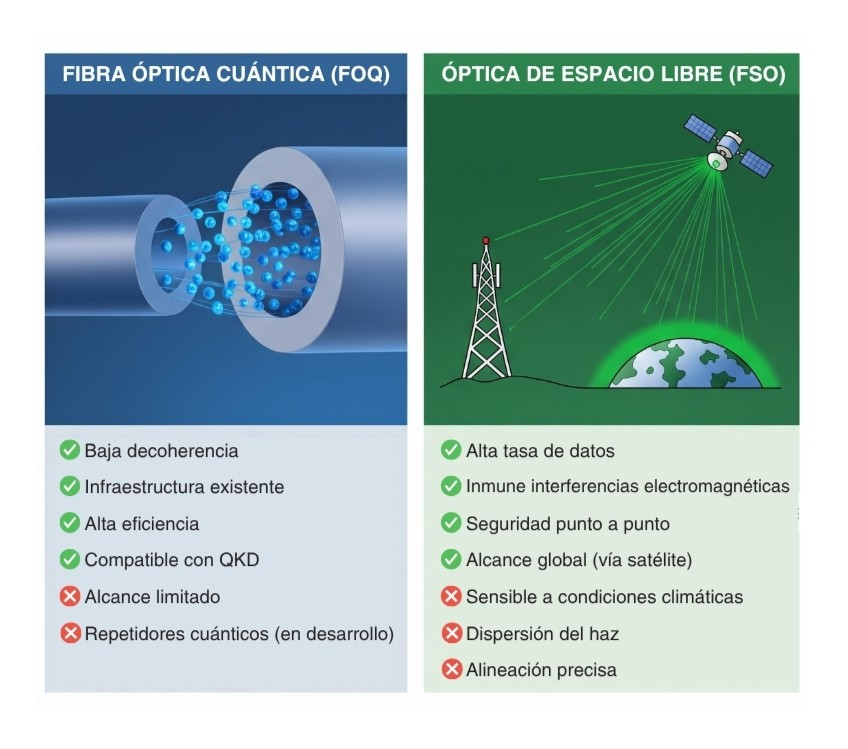
\includegraphics[width=0.7\textwidth]{pictures/FOQ_vs_FSO.jpg} 
\label{fig:redes_foq_vs_fso}
\end{figure}

\subsubsection{Internet Cuántico}
El Internet cuántico es una red mundial que permite el intercambio de información codificada en estados cuánticos, principalmente mediante el entrelazamiento de qubits entre usuarios remotos.

Uno de los trabajos pioneros en definir esta visión fue el artículo de H. J. Kimble en 2008~\cite{Kimble2008}, donde se esbozan los componentes necesarios para construir una red cuántica escalable: fuentes de entrelazamiento, repetidores cuánticos, memorias cuánticas robustas y nodos capaces de procesar, almacenar y reenviar qubits entrelazados. Según Kimble, estas capacidades no solo mejorarían la infraestructura actual, sino que darían lugar a un ecosistema cuántico interconectado, con aplicaciones científicas, tecnológicas y estratégicas sin precedentes.

No obstante, el desarrollo del Internet cuántico enfrenta retos técnicos y de ingeniería que van más allá de las limitaciones de hardware actual~\cite{Cacciapuoti2019}. Se trata de problemas complejos en cuanto a latencia, seguridad, gestión de recursos y limitaciones de ancho de banda. A diferencia del Internet clásico, donde los paquetes de datos pueden ser reenviados, almacenados o replicados sin pérdida de información, en el mundo cuántico esto no es posible debido al teorema de no clonación. Estas restricciones obligan a rediseñar por completo los protocolos de enrutamiento, sincronización y verificación de integridad, así como las capas de control que deben operar en redes distribuidas~\cite{Wehner2018}.

\subsection{Desafíos y Estrategias en el Nuevo Paradigma Cuántico}
\subsubsection{La Amenaza Cuántica}

En los últimos años, la narrativa del riesgo cuántico se ha consolidado en torno al concepto de Quantum Threats y el llamado Quantum Risk Horizon, es decir, el horizonte temporal a partir del cual la existencia de ordenadores cuánticos capaces de romper la criptografía tradicional se transforma de posibilidad teórica a amenaza práctica.

Ese punto crítico, donde la amenaza deja de ser potencial y se convierte en real, ha sido bautizado como Y2Q o Q-Day. El término Y2Q (Year to Quantum) representa el momento de incertidumbre en que un ordenador cuántico suficientemente potente logre romper los sistemas criptográficos actuales. 
	
Estudios recientes estiman que, en un plazo de 5 a 15 años, una computadora cuántica criptográficamente relevante (CRQC) podría descifrar cifrados estándar en menos de 24 horas~\cite{SANS2025}.

Un concepto clave en esta discusión es el teorema de Michele Mosca. Este teorema propone una sencilla fórmula de evaluación del riesgo: si el tiempo durante el cual los datos deben permanecer confidenciales (X) más el tiempo necesario para migrar a sistemas post-cuánticos seguros (Y) es mayor que el tiempo estimado para que los ordenadores cuánticos sean capaces de romper el cifrado (Z), entonces ya estamos en una zona de riesgo y la transición debe iniciarse de inmediato~\cite{Mosca2024}.

\begin{figure}[H]
\centering
\caption[Riesgo de Amenaza Cuántica]{
    \vspace{4pt}
    \fontsize{12}{11}\selectfont \\
    Riesgo de Amenaza Cuántica \\[2pt]
    \footnotesize Fuente: Elaboración propia
}
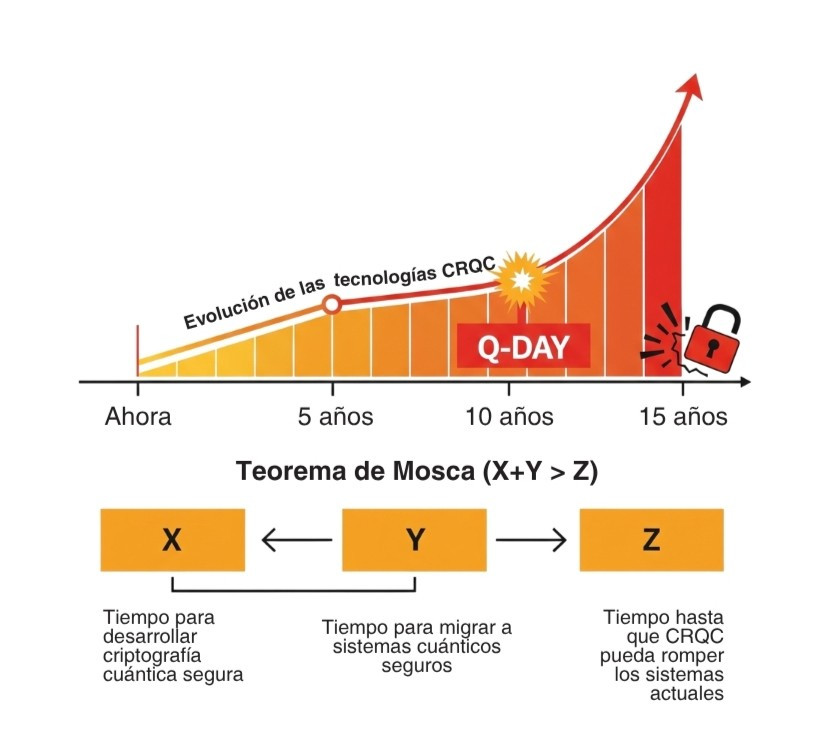
\includegraphics[width=0.7\textwidth]{pictures/Amenaza_cuantica.jpg} 
\label{fig:riesgo_amenaza_cuantica}
\end{figure}

Sin embargo la amenaza cuántica ya está presente a día de hoy. Muchas organizaciones, incluyendo actores maliciosos de tipo estatal, ya están empleando estrategias de “harvest now, decrypt later” (HNDL)~\cite{Adeola2025}, que consisten en recopilar masivamente datos cifrados con la esperanza de poder descifrarlos en el futuro cuando se tenga acceso a tecnología cuántica. Esto es especialmente alarmante para datos confidenciales como secretos industriales, patentes, documentos gubernamentales, información médica, comunicaciones diplomáticas, cuya filtración futura podría tener consecuencias catastróficas.

\subsubsection {Ataques Cuánticos de Nueva Generación}

La computación cuántica más allá del impacto sobre algoritmos criptográficos, está sentando las bases para una nueva generación de técnicas ofensivas de ataques completamente nuevas, donde el poder de procesamiento cuántico permite optimizar, acelerar o incluso hacer viables ciberataques que antes eran teóricamente inalcanzables.

Las técnicas de ataque clásicas como el escaneo de vulnerabilidades, fuzzing, evasión de detección, búsqueda de colisiones o los ataques por fuerza bruta podrían beneficiarse del uso de algoritmos cuánticos como Grover, diseñado para encontrar elementos en bases de datos no estructuradas con una velocidad cuadráticamente superior a la computación clásica, reduciendo de $O(N)$ a $O(\sqrt{N})$ el número de operaciones necesarias~\cite{Grover1996}. En un contexto ofensivo esta capacidad puede utilizarse para acelerar ataques de diccionario, identificar configuraciones débiles en redes, optimizar patrones de evasión contra sistemas de detección de intrusos (IDS)…
Este tipo de ataques aprovechan la velocidad cuántica para explorar con mayor eficiencia el espacio de ataques, reduciendo los tiempos y recursos necesarios para explotar sistemas.

Otra línea emergente es el desarrollo de malware asistido por computación cuantica (quantum-enhanced malware), que podría explotar vulnerabilidades en entornos de programación cuántica como Qiskit, Cirq o Braket, los cuales aún carecen de marcos de seguridad consolidados.

El uso ofensivo de algoritmos cuánticos de machine learning (QML)  abre una nueva dimensión en las fases de reconocimiento y recopilación de información previas a un ataque. Algoritmos cuánticos como Quantum Support Vector Machines (QSVM), Variational Quantum Classifiers (VQC), Quantum k-Nearest Neighbors (QkNN) pueden acelerar el procesamiento de grandes volúmenes de datos en registros de tráfico, logs de red, OSINT o metadatos de paquetes permitiendo identificar de forma eficiente debilidades operativas o topológicas en la infraestructura objetivo~\cite{Biamonte2016}. 

Un atacante equipado con capacidades QML, por ejemplo, evaluar múltiples rutas de ataque simultáneamente sobre una red objetivo incluso adaptarse dinámicamente a las defensas de un sistema, modificando el comportamiento ofensivo en tiempo real.

\subsubsection {Consideraciones estratégicas: soberanía digital y geopolítica cuántica}

La soberanía cuántica hace referencia a la capacidad de un Estado para desarrollar, controlar y proteger sus infraestructuras cuánticas críticas, sin depender de tecnologías o proveedores externos. 
	
Actualmente, el liderazgo cuántico está fuertemente concentrado en un pequeño número de países, con EE. UU., China dominando y, en menor medida, la Unión Europea. Esta asimetría tecnológica ha reactivado narrativas de competencia geopolítica similares a las vistas durante la carrera espacial del siglo XX, ahora centradas en el control de las “tecnologías cuánticas estratégicas”

La gestión de claves cuánticas, la confianza en dispositivos y las infraestructuras de red podrían convertirse en herramientas de poder blando o coercitivo, al igual que hoy ocurre con el control de cables submarinos, satélites GPS o infraestructuras 5G

La gestión de claves cuánticas, la verificación de dispositivos y el diseño de infraestructuras cuánticas de red tienen el potencial de convertirse en instrumentos de influencia geopolítica, al igual que esta pasando hoy en día con el control actual de cables submarinos, constelaciones satelitales o redes 5G. Países que lideren estos sectores podrían imponer sus estándares técnicos, normativos o comerciales.

La ausencia de un marco internacional de gobernanza cuántica añade incertidumbre al panorama. Aunque existen iniciativas multilaterales como el Quantum Flagship de la UE, el National Quantum Initiative Act de EE. UU. o propuestas en la ONU para limitar el uso militar de tecnologías cuánticas, aún no se ha definido un tratado global que regule el uso responsable de estas capacidades~\cite{PostQuantum2025}.

\subsection {Horizontes y Aplicaciones Emergentes del Ecosistema Cuántico}
Las tecnologías cuánticas están dando lugar a un conjunto de aplicaciones emergentes que podrían transformar numerosos sectores estratégicos. Aunque gran parte de la atención inicial se ha centrado en su impacto en criptografía o comunicaciones, sus implicaciones van mucho más allá.

En el ámbito biomédico y farmacéutico, la computación cuántica propone revolucionar la simulación molecular, permitiendo modelar proteínas, reacciones químicas complejas y compuestos bioactivos con un nivel de precisión y velocidad inalcanzables mediante métodos clásicos. Esta capacidad podría acelerar significativamente el desarrollo de nuevos medicamentos, terapias personalizadas y diagnósticos avanzados. Empresas como IBM Quantum colaboran con centros de investigación en proyectos de descubrimiento molecular asistido por algoritmos cuánticos~\cite{ClevelandClinic2024}.

En el ámbito de los materiales y la energía, los simuladores cuánticos están siendo utilizados para diseñar superconductores, catalizadores industriales o nuevos compuestos energéticos. Estas capacidades pueden tener un impacto directo en sectores como las energías renovables, la industria aeroespacial o el almacenamiento energético avanzado.

La optimización cuántica está encontrando aplicaciones en logística, transporte y finanzas. Algoritmos como el Quantum Approximate Optimization Algorithm (QAOA), el Quantum Annealing o el Vehicle Routing Problem (VRP) permiten abordar problemas de planificación, gestión de riesgos con una eficiencia muy superior a los métodos clásicos~\cite{Phillipson2024}. Estos avances están siendo explorados por empresas como Volkswagen, Goldman Sachs o Airbus.

Lejos de sustituir las tecnologías clásicas, la cuántica las complementan y amplifica, dando forma a un nuevo paradigma tanto tecnológico como económico en el que la computación, el procesamiento de datos, la simulación científica y la toma de decisiones podrían redefinir por completo los fundamentos actuales.
